%%%%%%%%%%%%%%%%%%%%%%%%%%%%%%%%%%%%%%%%%%%%%%%%%%%%%%%%%%%%%%%%%%%%%%%%%%%%%%%%
\chapter{Εισαγωγή}

Πολλοί παράγοντες συμβάλλουν στη συντονισμένη κίνηση του σώματος και η γοητεία της έχει οδηγήσει τους επιστήμονες σε αμέτρητα πειράματα και μελέτες ώστε να μπορέσουν να την εξηγήσουν. Ως αποτέλεσμα υπάρχει πλήθος υλικού και αποτελεσμάτων από τις μελέτες των χαρακτηριστικών των μυών, της γεωμετρικής τους συσχέτισης με τα οστά και την κίνηση των αρθρώσεων. Κατά καιρούς έχουν γίνει κλινικές μελέτες σε ασθένειες όπως είναι η εγκεφαλική παράλυση, το εγκεφαλικό επεισόδιο, η οστεοαρθρίτιδα και η Νόσος του Πάρκινσον, ώστε να μελετηθούν οι νευρικές διεγέρσεις που οδηγούν την κίνηση του σώματος τόσο πριν την θεραπεία αλλά και μετά, με σκοπό να εξαχθούν συμπεράσματα για την αντιμετώπιση τους. Δυστυχώς, η σύνθεση των δεδομένων από τις κλινικές μελέτες για την κατανόηση της δυσλειτουργίας που οφείλεται στην ασθένεια και η δημιουργία μιας επιστημονικής βάσης για την αντιμετώπιση της ανώμαλης κίνησης παραμένουν σημαντικές προκλήσεις.

Η χρήση πειραμάτων για την κατανόηση της δυναμικής της κίνησης έχει κάποια μειονεκτήματα. Για παράδειγμα η εκτίμηση των δυνάμεων που παράγονται από τους μύες είναι ακατόρθωτο να μετρηθούν πειραματικά με χρήση εξωτερικών οργάνων, λόγω του ότι είναι μη πρακτικό και χρονοβόρο. Επίσης υπάρχει δυσκολία κατανόησης των φαινομένων δράσης-αντίδρασης σε τόσο πολύπλοκα συστήματα μόνο από πειράματα. Ο προσδιορισμός της συνεισφοράς κάθε μυ στην κίνηση δεν είναι προφανής γιατί πολλές φορές η δράση του δεν συνεπάγεται μόνο την επιτάχυνση της άρθρωσης στην οποία δρα \cite{zajac-gordon89}, αλλά και άλλων αρθρώσεων.

Απαραίτητη προϋπόθεση για την μελέτη πολύπλοκων διατάξεων είναι η ανάπτυξη θεωρητικών μοντέλων που μπορούν να προσεγγίσουν τις ανθρώπινες δραστηριότητες και ο συνδυασμός αυτών με πειραματικές ενδείξεις. Το σύστημα θα πρέπει να είναι σε θέση να αναδείξει τις εξαρτήσεις μεταξύ του νευρικού, του μυικού, του σκελετικού συστήματος και της κίνησης του σώματος. Είναι φανερό ότι τα αποτελέσματα αυτού του είδους αναλύσεων παρέχουν μεγαλύτερη πληροφορία και δίνουν την δυνατότητα στους ερευνητές να εξάγουν κατάλληλη θεραπεία για την ασθένεια.

Τα τελευταία χρόνια και ιδιαίτερα με την ανάπτυξη των υπολογιστών είμαστε σε θέση να εκτελέσουμε πολύπλοκες προσομοιώσεις σε χρονικό διάστημα της τάξεως μερικών ωρών που πριν μια δεκαετία θα χρειαζόταν και μέρες. Η δραματική μείωση του χρόνου δεν οφείλεται μόνο στην ανάπτυξη των υπολογιστών, αλλά και στην εφεύρεση νέων πιο αποδοτικών μεθόδων. Η δυναμική προσομοίωση, η ανάπτυξη μυοσκελετικών και νευρομυοσκελετικών μοντέλων είναι σε θέση να δώσουν λύση σε πολλά προβλήματα που απασχολούν την ιατρική και είναι ευρέως αποδεκτά και έχουν μελετηθεί σε βάθος \cite{thelen-chumanov06, piazza06, pandy01, zajac02}.

Παρόλα αυτά υπάρχουν πολλά προβλήματα και φαινόμενα που δεν έχουν μοντελοποιηθεί ώστε να δώσουν πρόγνωση. Τα μοντέλα που έχουν δημιουργηθεί δεν είναι τόσο ακριβή και υπάρχει περιθώριο βελτιώσεων. Επίσης κάποιες αναλύσεις εκτελούνται ακόμα σε απαγορευτικούς χρόνους, καθιστώντας τις ακατάλληλες πολλές φορές. Μεγάλη πρόοδος έχει γίνει στην ανάπτυξη αξιόπιστων μοντέλων για τον μυ, ωστόσο λόγω της μεγάλης διαφοροποίησης που υπάρχει στο ανθρώπινο σώμα η χρήση ενός γενικού μοντέλου είναι δύσκολη. Από την άλλη πλευρά, υπάρχει μεγάλο χάσμα στην σύνδεση του νευρικού συστήματος με το κινητικό σύστημα, ενώ τα μοντέλα που υπάρχουν είναι απλοποιημένα και δεν αναπαριστούν πλήρως τις λειτουργίες τους. Συμπερασματικά, απαιτείται πολύ δουλεία τόσο από τους επιστήμονες που μελετούν την ανθρώπινη φυσιολογία, όσο και από τους μηχανικούς που μοντελοποιούν τα συστήματα προσομοιώσεων.

Είναι αναγκαία η δημιουργία κοινών εργαλείων και μοντέλων που θα χρησιμοποιούνται από την επιστημονική κοινότητα. Πολλά εργαστήρια έχουν αναπτύξει ενδιαφέρουσες τεχνικές, ωστόσο τα αποτελέσματα τους δεν είναι διαθέσιμα για να χρησιμοποιηθούν από τρίτους. Υπάρχουν αρκετά εμπορικά εργαλεία (\eng{Anybody, Adams, Visuals 3D}) που είναι ιδιόκτητου-κλειστού κώδικα και συνεπώς δεν δίνουν την δυνατότητα επέκτασης και ευελιξίας. Η ανάγκη αυτή έχει οδηγήσει στην ανάπτυξη του ανοιχτού συστήματος \eng{OpenSim} που υποστηρίζεται από μια μεγάλη κοινότητα με πολλά μοντέλα και αναλυτικές μεθόδους, έχοντας βοηθήσει σημαντικά τους ερευνητές τα τελευταία χρόνια. Δίνοντας την δυνατότητα στους επιστήμονες να μοιράζονται κοινές μεθόδους ανάλυσης, μοντέλα και αποτελέσματα, βοηθάει στην βελτίωση, στην αναπαραγωγή και στην επιβεβαίωση των αποτελεσμάτων που έχουν εξαχθεί από τρίτους.

%%%%%%%%%%%%%%%%%%%%%%%%%%%%%%%%%%%%%%%%%%%%%%%%%%%%%%%%%%%%%%%%%%%%%%%%%%%%%%%%
\section{Εφαρμογές}

Ως κλασικό παράδειγμα θα αποδείξουμε ότι τα μυοσκελετικά μοντέλα μπορούν να χρησιμοποιηθούν για να εκτιμηθεί η πορεία θεραπείας ορθοπεδικών εγχειρήσεων. Η βάδιση με λυγισμένα τα γόνατα (\eng{crouch gait}) είναι μια από τις πιο κοινές ανωμαλίες σε άτομα με εγκεφαλική παράλυση. Χαρακτηριστικό αυτής της βάδισης είναι η ανικανότητα παραγωγής αρκετής δύναμης από τους μύες στο γόνατο ώστε να σηκωθεί η λεκάνη μια κίνηση που απαιτεί πολύ δύναμη και κόπωση από τους μύες.  Μια αιτία είναι το μικρό μήκος του ημιτενοντώδους μυ και μερικές φορές η θεραπεία συνίσταται στην επιμήκυνση του. Ωστόσο μπορούν να υπάρχουν και άλλες αιτίες για την υπερβολική κάμψη του γονάτου (π.χ. αδύναμοι καμπτήρες της ποδοκνημικής άρθρωσης), και η επιμήκυνση του ημιτενοντώδους μπορεί να θέσει σε κίνδυνο την αντοχή των μυών στον αστράγαλο \cite{arnolda06}.

\begin{figure}[H]
    \centering
    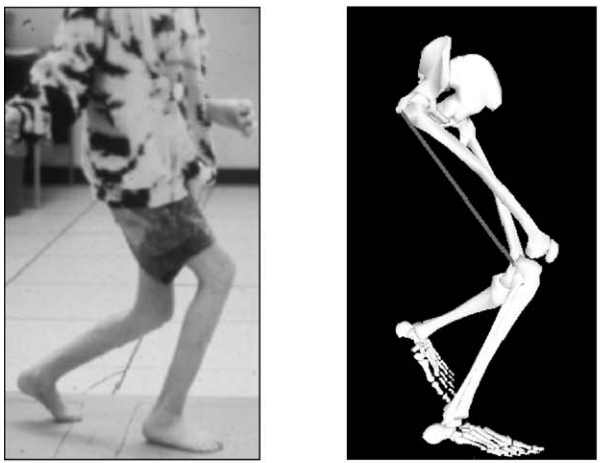
\includegraphics[width=0.8\textwidth, keepaspectratio]{fig/crouch-gait.png}
    \caption{Πρόβλημα βάδισης με λυγισμένα γόνατα \cite{arnolda06}}
    \label{fig:crouch-gait}
\end{figure}

Για αυτό το λόγο μπορούν να γίνουν καταγραφές της βάδισης του ασθενή σε ειδικά εργαστήρια και σε συνδυασμό με κατάλληλο μοντέλο των κάτω άκρων, ώστε να μελετηθεί για τον συγκεκριμένο ασθενή αν πρέπει να γίνει η επιμήκυνση του ημιτενοντώδους. Επίσης είναι δυνατή η παραμετροποίηση των μυών για το συγκεκριμένο ασθενή ώστε να μελετηθεί με ορθή δυναμική το αποτέλεσμα της εγχείρισης εικονικά. Τέτοιου είδους αναλύσεις θα ήταν ένα χρήσιμο εργαλείο για τους ιατρούς ώστε να τους δώσουν μια εποπτική κατάσταση του ασθενή, να βελτιώσουν την επιτυχία της εγχείρισης αλλά και την δημιουργία μιας θεραπευτικής αγωγής.

Ως δεύτερο παράδειγμα \cite{fregly07} είναι η μελέτη τρόπου βαδίσματος ώστε να μειωθεί η καταπόνηση του γονάτου. Σε αυτή την μελέτη οι ασθενείς με προβλήματα οστεοαρθρίτιδας καταπονούν το γόνατο κατά την βάδιση, οπότε οι συγγραφείς προτείνουν μια πολύ απλή παραλλαγή της βάδισης ώστε να μειωθεί η δύναμη που ασκείται στο γόνατο, στρέφοντας ελαφρά το πόδι προσταέξω. Κατά το πείραμα οι ασθενείς καταγράφονται από συστήματα παρακολούθησης της κίνησης ενώ μετράται και η αντίδραση εδάφους. Εφαρμόζεται αντίστροφη κινηματική και αντίστροφη δυναμική ώστε σε πραγματικό χρόνο υπάρχει μέτρηση της δύναμης που ασκείται στο γόνατο, αλλά και του προσανατολισμού του ποδιού. Στα πλαίσια του πειράματος έχει αναπτυχθεί μια συσκευή που σηματοδοτεί τον ασθενή όταν δεν ακολουθεί τους κανόνες της βάδισης για την μείωση της καταπόνησης. Ως αποτέλεσμα μετά από τέσσερα σεμινάρια οι ασθενείς είχαν συνηθίσει στο νέο τρόπο βάδισης και μείωσαν την καταπόνηση στο γόνατο.

\begin{figure}[H]
    \centering
    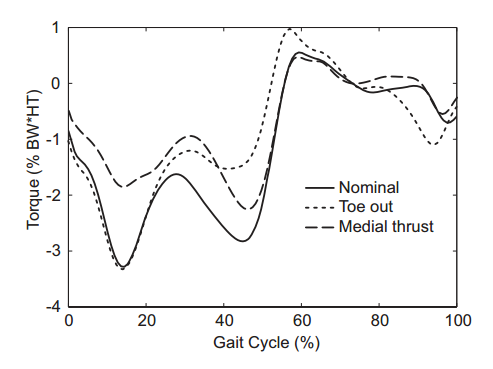
\includegraphics[width=0.8\textwidth, keepaspectratio]{fig/knee-load.png}
    \caption{Αποτελέσματα της παραγόμενης ροπής στο γόνατο \cite{fregly07}}
    \label{fig:knee-load}
\end{figure}

Σαν τρίτο παράδειγμα, θα ήταν ενδιαφέρον να μπορούσαμε να μελετήσουμε την συμπεριφορά των φαρμάκων στις ασθένειες κατά την δραστηριότητα των ανθρώπων. Ως βασικό προαπαιτούμενο απαιτείται η κατανόηση και η μοντελοποίηση της δράσης του φαρμάκου ώστε να μπορεί να προσομοιωθεί. Επίσης απαιτείται η μοντελοποίηση της ασθένειας και της σύνδεσής της με τις δραστηριότητες του ανθρώπου. Έχουν γίνει μελέτες μοντελοποίησης φαρμάκων όπως είναι η ντοπαμίνη για την θεραπεία της νόσου του Πάρκινσον \cite{haeri05}. Ωστόσο, υπάρχουν δυσκολίες όπως είναι η μοντελοποίηση των βασικών γαγγλίων (\eng{basal ganglia}). Παρόλα αυτά μπορούν να εξαχθούν ενδιαφέροντα αποτελέσματα και να εξηγηθούν φαινόμενα που ίσως οδηγήσουν στην εύρεση μεθόδων θεραπείας δύσκολων ασθενειών.

Συμπερασματικά, οι προσομοιώσεις μπορούν να βοηθήσουν την επιστήμη της ιατρικής και όχι μόνο στη μελέτη της συμπεριφοράς μιας ασθένειας, αλλά και στην εξαγωγή συμπερασμάτων για τη θεραπεία και τις στρατηγικές αγωγής. Οι μέθοδοι προσομοιώσεων χρησιμοποιούνται σε άλλους τομείς, όπως είναι η βιομηχανία των αυτοκινήτων για την σχεδίαση κινητήρων όπου έχει μειωθεί δραματικά το κόστος κατασκευής τους. Ως εκ τούτου δείχνει ελπιδοφόρα η εφαρμογή τους και στην ιατρική, στην παραγωγή νέων φαρμάκων, την δημιουργία νέων ορθοπεδικών μηχανημάτων όπως είναι οι υποστηρικτές σκελετικού συστήματος \cite{stopforth12} και σε πολλούς άλλους κλάδους.

%%%%%%%%%%%%%%%%%%%%%%%%%%%%%%%%%%%%%%%%%%%%%%%%%%%%%%%%%%%%%%%%%%%%%%%%%%%%%%%%
\section{Σχετική Βιβλιογραφία}

Οι μυικές δυνάμεις κατά την διεξαγωγή μιας κίνησης είναι αδύνατον να καταγραφούν εύκολα πειραματικά σε κλινικές μελέτες. Η μεγάλη ανακάλυψη τα τελευταία χρόνια είναι η δυνατότητα εκτίμησης της συνεισφοράς κάθε μυ σε συγκεκριμένη κίνηση απευθείας από την καταγεγραμμένη κίνηση, που είναι και ο κλασικός τρόπος εξαγωγής αποτελεσμάτων \cite{hamner10, mclean03}. Η αντίστροφη δυναμική έχει γίνει ρουτίνα σε κλινικές αναλύσεις της βάδισης, υπολογίζοντας τις ροπές που ασκούνται στις αρθρώσεις κατά την δοσμένη κίνηση, ωστόσο απαιτεί γνώση των εξωτερικές δυνάμεων που ασκούνται στο σύστημα. Η μέθοδος της στατικής βελτιστοποίησης (\eng{static optimization}) σε συνδυασμό με τα αποτελέσματα της αντίστροφης δυναμικής είναι σε θέση να εκτιμήσει την συνεισφορά κάθε μυ \cite{heintz06, erdemir07} και χρησιμοποιείται εδώ και δεκαετίες.

Η δυσκολία απόκτησης πειραματικών δεδομένων, αλλά και το σφάλμα που εισάγει η αντίστροφη δυναμική, οδήγησε την ερευνητική κοινότητα σε εναλλακτικές μεθόδους με χρήση της ορθής δυναμικής \cite{buchanan04}. Παρόλο που η ορθή δυναμική απαιτεί ολοκληρώσεις και γενικά είναι υπολογιστικά πιο ακριβή, έχουν αναπτυχθεί ενδιαφέρουσες μεθόδοι ανάλυσης. Δεδομένα που μπορούν να χρησιμοποιηθούν και να βελτιώσουν το αποτέλεσμα της ορθής δυναμικής είναι οι καταγεγραμμένες διεγέρσεις μυών μέσω \eng{EMG}, μυικές δυνάμεις οι οποίες μπορούν να μετρηθούν με διάφορα όργανα και οι ροπές στις αρθρώσεις. Σε περίπτωση που δεν γνωρίζουμε τις εξωτερικές δυνάμεις που δρουν στην διάταξη, μπορούν να εισαχθούν πολύ εύκολα στις εξισώσεις ως περιορισμοί και να εκτιμηθούν κατά την διάρκεια των προσομοιώσεων \cite{hamner10, seitha11}. Πολλές φορές δεν είναι γνωστές οι είσοδοι του συστήματος, οπότε σε τέτοιες περιπτώσεις διεγείρεται το σύστημα ελαφρώς, εκτελείται η ορθή δυναμική ώστε να εκτιμηθεί το αποτέλεσμα και στην συνέχεια γίνεται βελτιστοποίηση των εισόδων μέχρι να παραχθεί το επιθυμητό αποτέλεσμα \cite{pandy01}. Αυτές οι μέθοδοι βασίζονται στην θεωρία του βέλτιστου έλεγχου και η επιλογή κατάλληλων κριτηρίων βελτιστοποίησης εξειδικεύεται ανάλογα με την εφαρμογή. Μια άλλη κατηγορία μεθόδων είναι αυτές της παρακολούθησης (\eng{forward dynamics assisted data tracking}). Αρχικά τροφοδοτείται κατάλληλα το σύστημα της ορθής δυναμικής ώστε να εκτιμηθεί το αποτέλεσμα και σε συνδυασμό με ένα κλειστό βρόγχο γίνεται προσπάθεια να ελεγχθεί (μειωθεί) το σφάλμα μεταξύ της καταγεγραμμένης κίνησης και της εκτιμώμενης. Μια από τις πιο αποδοτικές μεθόδους που ανήκει σε αυτήν την κατηγόρια είναι ο υπολογισμός μυϊκών διεγέρσεων (\eng{computed muscle control}), που προτάθηκε από \cite{thelen06}.

Απαραίτητη προϋπόθεση ώστε να γίνει η ανάλυση και η εκτίμηση των μυϊκών δυνάμεων είναι η ύπαρξη μυοσκελετικών μοντέλων που συσχετίζουν την σκελετική δομή με την παραγόμενη δύναμη από τους μύες. Απαραίτητο στοιχείο αυτής της δομής είναι η σωστή μοντελοποίηση της δυναμικής του μυ. Τα μοντέλα μυών που χρησιμοποιούνται συνήθως στις προσομοιώσεις είναι τύπου \eng{Hill} και προτάθηκαν αρχικά από \cite{zajac89}, στην συνέχεια με μικρές τροποποίησες από \cite{thelen03} και η πιο πρόσφατη εργασία \cite{millard13}. Η τελευταία επιβεβαίωσε πειραματικά τα αποτελέσματα των μοντέλων και πρότεινε εναλλακτικό μοντέλο, το οποίο βελτιώνει κατά πολύ τον χρόνο εκτίμησης των δυνάμεων και συνεπώς τον χρόνο που απαιτεί η όλη διαδικασία, χωρίς να μειωθεί η ακρίβεια των υπολογισμών. Από την άλλη πλευρά είναι αναγκαία η διασύνδεση των μυϊκών δυνάμεων με τις δυναμικές εξισώσεις κίνησης και γι' αυτό απαιτείται η εισαγωγή της μυϊκής ροπής αδράνειας (\eng{muscle moment arm}) \cite{delp95}, η οποία συνδέει την ροπή της άρθρωσης με τους μύες που δρουν σε αυτήν. Τέλος, αφού υπάρχουν τα μαθηματικά εργαλεία το επόμενο βήμα είναι η γεωμετρική τοποθέτηση των μυών πάνω στο σκελετικό σύστημα με βάση την φυσιολογία του ανθρώπου.

Η καταγραφή της κίνησης είναι ένα δύσκολο πρόβλημα και υπάρχει πληθώρα λύσεων ανάλογα με την εφαρμογή. Ενδιαφέρον παρουσιάζει η εκτίμηση της θέσης των αρθρώσεων στο τρισδιάστατο χώρο, καθώς η παρακολούθηση της κίνησης περιγράφεται αποτελεσματικά από την παρακολούθηση των επιμέρους αρθρώσεων \cite{poppe07}. Οι αλγόριθμοι εκτίμησης της θέσης των αρθρώσεων συνήθως χρησιμοποιούν χάρτες βάθους που παρέχονται από συσκευές στερεοσκοπικής όρασης. Ένας από τους πιο αποτελεσματικούς αλγορίθμους εκτίμησης της θέσης των αρθρώσεων \cite{shotton11}, όσον αφορά την ταχύτητα παροχής αποτελεσμάτων εφαρμογή πραγματικού χρόνου και μορφολογική διαφοροποίηση ανθρώπινων χαρακτηριστικών είναι υλοποιημένος εσωτερικά στη συσκευή \eng{Kinect}. Το \eng{Kinect} είναι μια φθηνή συσκευή στερεοσκοπικής όρασης που είναι σε θέση να καταγράψει τις ανθρώπινες δραστηριότητες.

Η επιστημονική κοινότητα έχει αναπτύξει ενδιαφέρουσες μεθόδους ανάλυσης της δυναμικής συμπεριφοράς του ανθρώπου κατά την διεξαγωγή κινήσεων, ωστόσο πολλές φορές τα αποτελέσματα των ερευνών δεν είναι διαθέσιμα σε τρίτους. Επίσης υπάρχουν πολλές εμπορικές εφαρμογές που παρέχουν την τεχνογνωσία, ωστόσο είναι ακριβές και δεν διαθέτουν δυνατότητα προσαρμογής στις απαιτήσεις του χρήστη. Για τον λόγο αυτό αναπτύχθηκε τα τελευταία χρόνια μια βιβλιοθήκη-εφαρμογή με το όνομα \eng{OpenSim} για την διεξαγωγή των αναλύσεων, συγκεντρώνοντας τις πιο πρόσφατες ανακαλύψεις μεθόδων \cite{delp07}.

%%%%%%%%%%%%%%%%%%%%%%%%%%%%%%%%%%%%%%%%%%%%%%%%%%%%%%%%%%%%%%%%%%%%%%%%%%%%%%%%
\section{Συνεισφορά}

Η συνεισφορά της παρούσας διπλωματικής εργασίας αφορά στη διαδικασία καταγραφής της ανθρώπινης κίνησης με σχετικά φθηνό και αποτελεσματικό τρόπο, χρησιμοποιώντας τη συσκευή \eng{Kinect}. Λόγω του θορύβου της καταγεγραμμένης κίνησης μελετώνται κάποιες μέθοδοι ώστε να βελτιωθούν οι μετρήσεις με την απαλοιφή του θορύβου, βήμα απαραίτητο για την εξαγωγή ορθών αποτελεσμάτων στα μετέπειτα στάδια. Στη συνέχεια γίνεται μια μοντελοποίηση των κάτω άκρων του ανθρώπινου σώματος. Αρχικά αναπτύχθηκε ένα σκελετικό μοντέλο που περιγράφει τους βαθμούς ελευθερίας της διάταξης και είναι σε θέση να απαντήσει στα ερωτήματα που αφορούν την κατανομή δυνάμεων κατά την κίνηση. Ακολούθως εισάγονται τα μυοσκελετικά μοντέλα που βοηθούν στην εξαγωγή συμπερασμάτων σχετικά με την συνεισφορά των μυών στην συντονισμένη κίνηση. Το μοντέλο του μυ που χρησιμοποιήθηκε είναι τύπου \eng{Hill} και βασίζεται στην πρόσφατη εργασία \cite{millard13}, ενώ η διάταξη αποτελείται από 86 μύες συνολικά.

Με την παρουσία ενός μοντέλου σε συνδυασμό με την καταγεγραμμένη κίνηση είμαστε σε θέση να προχωρήσουμε στο κομμάτι της ανάλυσης και εξαγωγής αποτελεσμάτων. Απαραίτητη μέθοδος για την μεταφορά από την καταγεγραμμένη κίνηση σε κίνηση του μοντέλου είναι η αντίστροφη δυναμική. Προτού διεξαχθεί η μέθοδος πρέπει να εκτελεστούν κάποια απαραίτητα βήματα προετοιμασίας. Το πρώτο είναι η αντιστοίχιση των σημείων του μοντέλου και της πειραματικής κίνησης, τοποθετώντας κάποιες ενδείξεις. Δεύτερο βήμα, το οποίο βελτιώνει σημαντικά τα σφάλματα της αντίστροφης κινηματικής, είναι η κανονικοποίηση του γενικού μοντέλου που αναπτύχθηκε στα χαρακτηριστικά του συγκεκριμένου δείγματος (π.χ. το γενικό μοντέλο μπορεί να αφορά άνθρωπο ύψους δυο μέτρων, ενώ το υποκείμενο να είναι 1.6\eng{m}). Τέλος, εκτελείται η αντίστροφη κινηματική από την οποία λαμβάνονται οι συντεταγμένες του μοντέλου για την παραγωγή της καταγεγραμμένης κίνησης.

Μετά την αντίστροφη κινηματική είναι διαθέσιμα πλέον τα απαιτούμενα δεδομένα για τη δυναμική ανάλυση. Υπάρχουν δυο είδη τεχνικών που εξετάζονται στην συνέχεια, οι τεχνικές της αντίστροφης δυναμικής και οι τεχνικές της ορθής δυναμικής. Οι πρώτες είναι πιο γρήγορες και πιο εύκολες στην χρήση, ωστόσο εισάγουν σφάλματα. Οι δεύτερες είναι πιο αργές, αλλά δίνουν σημαντικό περιθώριο για την εφαρμογή κάποιων ενδιαφέροντων μεθόδων, οι οποίες δίνουν ορθά αποτελέσματα. Ως αποτέλεσμα της δυναμικής ανάλυσης είμαστε σε θέση να γνωρίζουμε τις ροπές και τις δυνάμεις που ασκούνται στις αρθρώσεις. Στην συνέχεια μπορούμε να συνεχίσουμε ένα βήμα πιο πέρα και να εξάγουμε συμπεράσματα για την μυϊκή συνεισφορά στην κίνηση. Οι μέθοδοι που εκτιμούν τις μυϊκές δυνάμεις και διεγέρσεις, λόγω της αδυναμίας εύρεσης μοναδικής λύσης, λαμβάνουν κάποια κριτήρια βελτιστοποίησης. Ως συνεισφορά της παρούσας εργασίας μελετούνται οι διάφορες τεχνικές που υπάρχουν και επιβεβαιώνονται με βάση την σχετική βιβλιογραφία για το παραγόμενο αποτέλεσμα και προτείνεται μια σειρά από στάδια ώστε να φτάσουμε σε αξιόπιστα αποτελέσματα.

